
\newpage
\subsection*{Задание 1: Измерение мощности постоянного тока косвенным методом при помощи вольтметра и амперметра.}

\vspace{1cm}

\begin{center}
		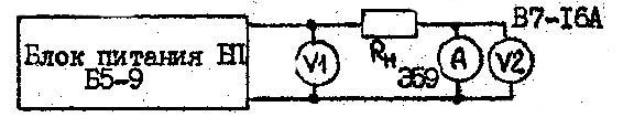
\includegraphics[width=0.6\textwidth]{ch1.jpg}\\
\end{center}

\vspace{1cm}

\textbf{Формулы для расчетов:}\\
\\
1. Измеренное значение мощности $P_{u}=U_{v1}*I_{a}$\\
2. Мощность, потребляемая амперметром $P_{a}=U_{v2}*I_{a}$\\
3. Мощность, рассеиваемую в нагрузке, определяют с учетом поправки $–P_{a}: P{n}=Р_{u}-P_{a}$\\
4. Относительная погрешность измерения мощности определяют по формуле\\

$\delta_{p}=\sqrt{\delta_{v1}^2 + \delta_{A}^2} = \sqrt{(\frac{I_{nom}*k_{A}}{I_{A}})^2 + (\frac{U_{nom}*k_{v1}}{U_{v1}})^2}$\\
\vspace{1cm}
\\
\textbf{Характеристики приборов:}\\
\\
$I_{nom}=0.05 А$\\
$U_{nom}=150 В$\\
$ka=0.5$\\
$kv_{1}=0.5$\\

\vspace{0.5cm}
\textbf{Расчеты:}
\\
1. \\
	$P_{u1}=20*0.044=0.88 W\\
	P_{u2}=20*0.019=0.38 W\\
 	P_{u3}=20*0.013=0.26 W\\
	P_{u4}=20*0.009=0.18 W$
\\
\\
2.\\
	$P_{а1}=0.774*0.44=0.034 W\\
	P_{а2}=0.399*0.019=0.008 W\\
	P_{а3}=0.279*0.013=0.004 W\\
	P_{а4}=0.201*0.009=0.002 W$
	\\
	\\
3. \\
	$P_{n1}=0.88-0.34=0.846 W\\
	P_{n2}=0.38-0.008=0.372 W\\
	P_{n3}=0.26-0.004=0.256 W\\
	P_{n4}=0.18-0.002=0.178 W$
	\\
	\\

\textbf{Результаты расчетов:}\\
$\delta_{1}=3.79\\
\delta_{2}=3.97\\
\delta_{3}=4.21\\
\delta_{4}=4.1$
\\
\vspace{1cm}
\begin{table}[h!]
	\begin{tabular}{|c|c|c|c|c|}
		\hline
		Напряжение $U_{v1}$, В 				&	20	&	20	&	20	&	20	\\
		\hline
		Сопротивление нагрузки $R_{n}$, Ом	&	500	&	1000&	1500&	2000\\
		\hline
		Ток нагрузки $I_{A}$, A 			&	0.44&  	0.019& 	0.013& 	0.009\\
		\hline
		Напряжение $U_{v2}$, В 				&	0.774&	0.399&	0.279&	0.201\\
		\hline
		Поправка - $P_{A}$, W				& 	0.034&	0.008&	0.004&	0.002\\
		\hline
		Мощность нагрузки $P_{H}$, W		&	0.846&	0.372&	0.256&	0.178\\
		\hline
		Относительная погрешность $\delta$, $\%$ & 	3.79&	3.97&	4.21&	4.1\\
		\hline	
	\end{tabular}
\end{table}

